\documentclass[10pt]{article}
\usepackage[polish]{babel}
\usepackage[utf8]{inputenc}
\usepackage[T1]{fontenc}
\usepackage{graphicx}
\usepackage[export]{adjustbox}
\graphicspath{ {./images/} }
\usepackage{amsmath}
\usepackage{amsfonts}
\usepackage{amssymb}
\usepackage[version=4]{mhchem}
\usepackage{stmaryrd}

\title{GIMNAZJUM }

\author{}
\date{}


\begin{document}
\maketitle
\begin{enumerate}
  \item Szkic przedstawia działkę prostokątną podzieloną łamaną ABCD na dwa kawałki. Odcinki AB, BC i CD są równoległe do boków prostokąta i w rzeczywistości mają długości odpowiednio 30 m, 24 m i 10 m. Łamaną ABCD chcemy zastąpić linią AE nie zmieniając pól tych dwóch kawałków. W jakiej odległości od punktu D\\
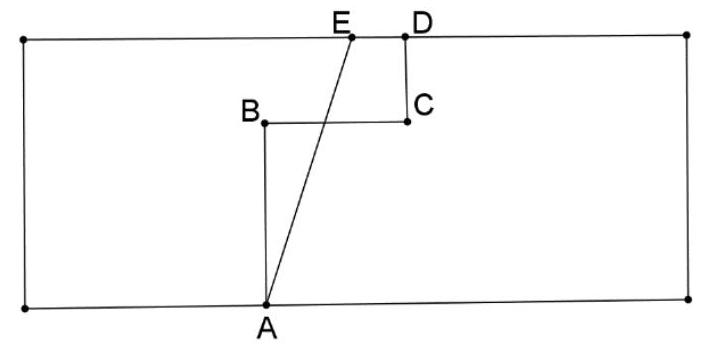
\includegraphics[max width=\textwidth, center]{2024_11_21_d3ff8dbf58272e4ef542g-1(1)}\\
znajduje się punkt E?
  \item Na ile sposobów można wybrać z szachownicy pole białe i czarne, by nie leżały one w tym samym wierszu ani w tej samej kolumnie?
  \item Trzy kwadraty tworzą prostokąt jak na rysunku. Policz miarę kąta CPE.\\
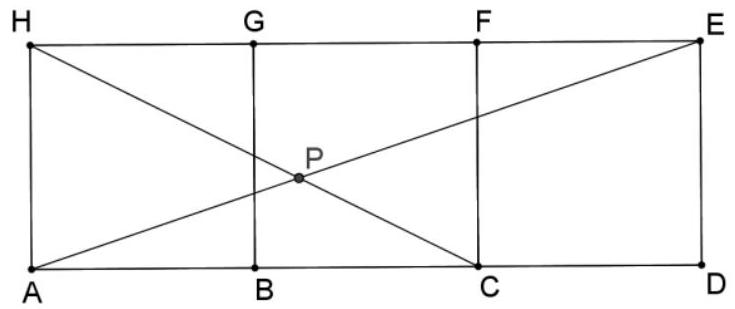
\includegraphics[max width=\textwidth, center]{2024_11_21_d3ff8dbf58272e4ef542g-1(2)}
\end{enumerate}

\section*{LICEUM}
\begin{enumerate}
  \item Dany jest kwadrat magiczny o wymiarach \(3 \times 3\). Dwie z jego liczb ujawniono na rysunku obok. Jaka liczba ukrywa się pod literą \(a\) ?
\end{enumerate}

\begin{center}
\begin{tabular}{|l|l|l|}
\hline
\(a\) &  &  \\
\hline
 &  & 33 \\
\hline
 & 25 &  \\
\hline
\end{tabular}
\end{center}

\begin{enumerate}
  \setcounter{enumi}{1}
  \item W prostokącie \(A B C D\) dwusieczna kąta CDA przecina przekątną AC w punkcie E. odległość punktu E od boku AB wynosi 1, a od boku BC wynosi 8 . Oblicz długość boku \(A B\).\\
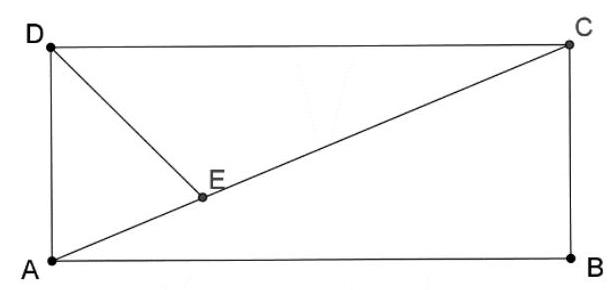
\includegraphics[max width=\textwidth, center]{2024_11_21_d3ff8dbf58272e4ef542g-1}
  \item Niech \(k=\frac{a}{b+c}=\frac{b}{a+c}=\frac{c}{a+b}\). Ile różnych wartości może przyjąć \(k\) ?
\end{enumerate}

\end{document}